\documentclass[oneside,a4paper,14pt]{extarticle}
\usepackage[a4paper,letterpaper,top=20mm,bottom=20mm,left=20mm,right=10mm]{geometry}
\usepackage[russian]{babel}
\usepackage{textcomp}
\usepackage{indentfirst}
\usepackage{graphicx}
\usepackage{mwe}
\usepackage{wrapfig}
\usepackage{caption}
\usepackage{amsmath}
\usepackage{amsfonts}
\usepackage{amsthm}
\usepackage{amssymb}
\usepackage[all]{xy}
\usepackage[breaklinks]{hyperref}
\usepackage{titlesec}
\usepackage{xcolor}
\usepackage{nicematrix}
\usepackage{multirow}
\usepackage{tikz}

\titleformat{\section} % Настройка формата заголовков секций
{\normalsize\bfseries} % Устанавливает размер шрифта на нормальный и делает его жирным
{\thesection} % Указывает, что номер секции будет отображаться перед заголовком
{1em} % Устанавливает расстояние между номером секции и заголовком в 1em
{} % Дополнительные параметры.

\titleformat{\subsection} % Настройка формата заголовков подсекций
{\normalsize\bfseries} % Устанавливает размер шрифта на нормальный и делает его жирным
{\thesubsection} % Указывает, что номер подсекции будет отображаться перед заголовком
{1em} % Устанавливает расстояние между номером подсекции и заголовком в 1em
{} % Дополнительные параметры.

\titleformat{\subsubsection} % Настройка формата заголовков подподсекций
{\normalsize\bfseries} % Устанавливает размер шрифта на нормальный и делает его жирным
{\thesubsection} % Указывает, что номер подподсекции будет отображаться перед заголовком
{1em} % Устанавливает расстояние между номером подподсекции и заголовком в 1em
{} % Дополнительные параметры.

\renewcommand\baselinestretch{1.45}\normalsize %межстр интервал
\setlength{\parindent}{1.25cm} %длина отступа нового абзаца

\begin{document}
\newpage
\thispagestyle{empty}
\begin{center}
	МИНИСТЕРСТВО НАУКИ И ВЫСШЕГО ОБРАЗОВАНИЯ\\
	РОССИЙСКОЙ ФЕДЕРАЦИИ
	ФЕДЕРАЛЬНОЕ ГОСУДАРСТВЕННОЕ БЮДЖЕТНОЕ\\
	ОБРАЗОВАТЕЛЬНОЕ
	УЧРЕЖДЕНИЕ ВЫСШЕГО ОБРАЗОВАНИЯ\\
	«ВЯТСКИЙ ГОСУДАРСТВЕННЫЙ УНИВЕРСИТЕТ»\\
	Институт математики и информационных систем\\
	Факультет автоматики и вычислительной техники\\
	Кафедра электронных вычислительных машин
\end{center}
\vspace{20mm}

\begin{center}
	Отчёт по лабораторной работе №7\\
	по дисциплине\\
	<<Информатика>>\\
	<<Построение комбинационных схем.>>\\
\end{center}
\vspace{40mm}
\noindent
\begin{tabular}{ll}
	Разработал студент гр. ИВТб-1301-05-00 & \rule[-1mm]{30mm}{0.10mm}\,/Черкасов А. А./ \\
	                                       & \hspace{8mm}\footnotesize(подпись)          \\

	Проверил доцент кафедры ЭВМ            & \rule[-1mm]{30mm}{0.10mm}\,/Коржавина А.С./ \\
	                                       & \hspace{8mm}\footnotesize(подпись)          \\
\end{tabular}

\vfill
\begin{center}
	Киров\\
	2024
\end{center}

\newpage\thispagestyle{plain}
\section*{Цель работы}
Цель работы: Закрепить на практике знания о минимизации системы булевых функций
и получить навыки реализации простейших арифметических устройств.

\section*{Задания}
\begin{enumerate}
	\item
	      Выполнить минимизацию булевых функций, представить функции
	      различных базисах --- основном логическом базисе (И, ИЛИ, НЕ) или в
	      базисе Шеффера (И-НЕ).
	\item
	      Построить четырехразрядный полный сумматор, складывающий 2
	      двоичных четырехразрядных числа и учитывающий единицу переноса.
	\item
	      Построить четырехразрядный умножитель, перемножающий 2 двоичных
	      четырехразрядных числа.
	\item
	      Построить 16-разрядный сумматор со схемами ускоренного переноса.
\end{enumerate}
\newpage

\section*{Решение}
\noindent\textbf{Задание 1}\\
\noindent Значения функций $F_1$ и $F_2$ приведены в таблице 1.\\
\begin{flushleft}
	Таблица 1 – Значения функций 1 и 2.\\
	\begin{NiceTabular}{|c|c|c|c|c|}[colortbl-like]
		\hline
		$x_1$ & $x_2$ & $x_3$ & $F_1$ & $F_2$ \\ \hline
		0     & 0     & 0     & 0     & 1     \\ \hline
		0     & 0     & 1     & 0     & 1     \\ \hline
		0     & 1     & 0     & 1     & 0     \\ \hline
		0     & 1     & 1     & 1     & 0     \\ \hline
		1     & 0     & 0     & 1     & 0     \\ \hline
		1     & 0     & 1     & 0     & 0     \\ \hline
		1     & 1     & 0     & 0     & 1     \\ \hline
		1     & 1     & 1     & 0     & 1     \\ \hline
	\end{NiceTabular}
\end{flushleft}
\noindent Диаграмма Вейча-Карно для $F_1$ приведена в Таблице 2.
\begin{flushleft}
	Таблица 2 – Диаграмма Вейча-Карно для $F_1$\\
	\begin{NiceTabular}{|c|c|c|c|c|}[colortbl-like]
		\hline
		$x_1 \backslash x_2 x_3$ & 00 & 10 & 11 & 01 \\ \hline
		0                        & 0  & 1  & 1  & 0  \\ \hline
		1                        & 1  & 0  & 0  & 0  \\ \hline
	\end{NiceTabular}
\end{flushleft}
$F_1 =  \overline{x_1}  \cdot x_3+x_1 \cdot  \overline{x_2}  \cdot  \overline{x_3} $~\\
\noindent Схема $F_1$ приведена на Рисунке 1.\\
\begin{figure}[h!]
	\centering
	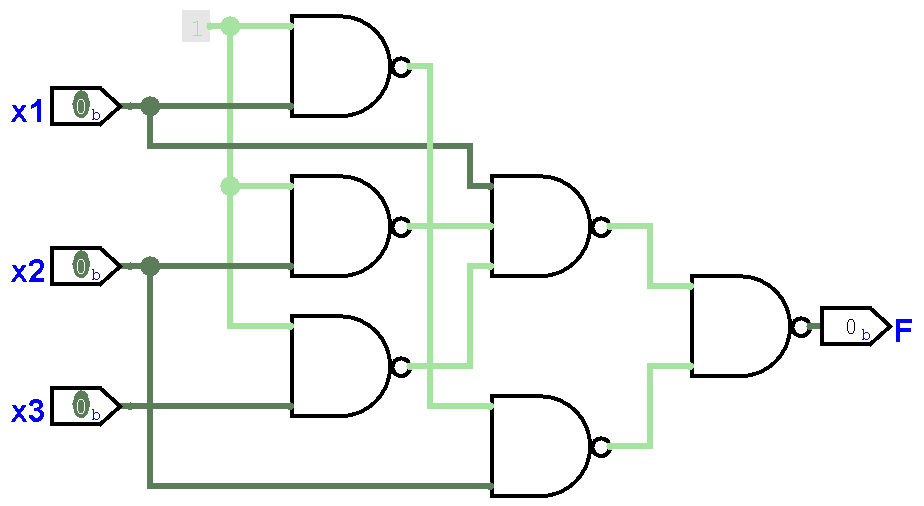
\includegraphics[width=0.5\textwidth]{pics/1f.png}
	\caption*{Рисунок 1 - Схема $F_1$.}
\end{figure}
\newpage
\noindent Диаграмма Вейча-Карно для $F_2$ приведена в Таблице 3.
\begin{flushleft}
	Таблица 3 – Диаграмма Вейча-Карно для $F_2$\\
	\begin{NiceTabular}{|c|c|c|c|c|}[colortbl-like]
		\hline
		$x_1 \backslash x_2 x_3$ & 00 & 10 & 11 & 01 \\ \hline
		0                        & 1  & 1  & 0  & 0  \\ \hline
		1                        & 0  & 0  & 1  & 1  \\ \hline
	\end{NiceTabular}
\end{flushleft}
$F_2 =  \overline{x_1}  \cdot  \overline{x_2} + x_1 \cdot x_2$~\\
\noindent Схема $F_2$ приведена на Рисунке 2.\\
\begin{figure}[h!]
	\centering
	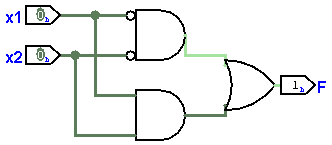
\includegraphics[width=0.5\textwidth]{pics/2f.png}
	\caption*{Рисунок 2 - Схема $F_2$.}
\end{figure}
\newpage
\noindent Значения функций $F_3$ и $F_4$ приведены в таблице 4.
\begin{flushleft}
	Таблица 4 – Значения функций 3 и 4.\\
	\begin{NiceTabular}{|c|c|c|c|c|c|}[colortbl-like]
		\hline
		$x_1$ & $x_2$ & $x_3$ & $x_4$ & $F_3$ & $F_4$ \\ \hline
		0     & 0     & 0     & 0     & 1     & 1     \\ \hline
		0     & 0     & 0     & 1     & 1     & 1     \\ \hline
		0     & 0     & 1     & 0     & 0     & 0     \\ \hline
		0     & 0     & 1     & 1     & 0     & 0     \\ \hline
		0     & 1     & 0     & 0     & 0     & 1     \\ \hline
		0     & 1     & 0     & 1     & 1     & 0     \\ \hline
		0     & 1     & 1     & 0     & 1     & 0     \\ \hline
		0     & 1     & 1     & 1     & 0     & 0     \\ \hline
		1     & 0     & 0     & 0     & 1     & 1     \\ \hline
		1     & 0     & 0     & 1     & 1     & 0     \\ \hline
		1     & 0     & 1     & 0     & 0     & 1     \\ \hline
		1     & 0     & 1     & 1     & 0     & 0     \\ \hline
		1     & 1     & 0     & 0     & 1     & 1     \\ \hline
		1     & 1     & 0     & 1     & 0     & 1     \\ \hline
		1     & 1     & 1     & 0     & 0     & 0     \\ \hline
		1     & 1     & 1     & 1     & 1     & 1     \\ \hline
	\end{NiceTabular}
\end{flushleft}
\noindent Диаграмма Вейча-Карно для $F_3$ приведена в Таблице 5.
\begin{flushleft}
	Таблица 5 – Диаграмма Вейча-Карно для $F_3$\\
	\begin{NiceTabular}{|c|c|c|c|c|}[colortbl-like]
		\hline
		$x_1 x_2 \backslash x_3 x_4$ & 00 & 10 & 11 & 01 \\ \hline
		00                           & 1  & 0  & 0  & 1  \\ \hline
		10                           & 1  & 0  & 0  & 1  \\ \hline
		11                           & 1  & 0  & 1  & 0  \\ \hline
		01                           & 0  & 1  & 0  & 1  \\ \hline
	\end{NiceTabular}
\end{flushleft}
$F_3 =  \overline{x1}  \cdot  \overline{x4} +x1 \cdot  \overline{x2}  \cdot  \overline{x3}  \cdot x4+ \overline{x2}  \cdot x3 \cdot  \overline{x4} +x2 \cdot  \overline{x3}  \cdot  \overline{x4} +x1 \cdot x2 \cdot x3 \cdot x4$~\\
\noindent Схема $F_3$ приведена на Рисунке 3.\\
\begin{figure}[h!]
	\centering
	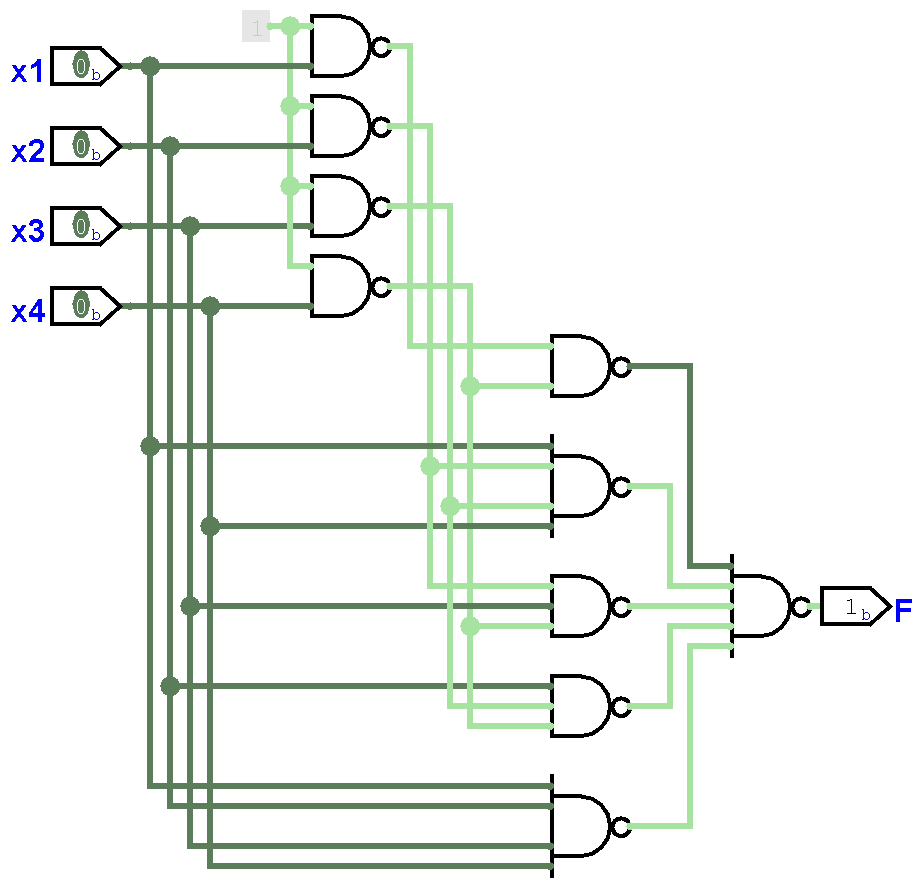
\includegraphics[width=0.5\textwidth]{pics/3f.png}
	\caption*{Рисунок 3 - Схема $F_3$.}
\end{figure}
\newpage
\noindent Диаграмма Вейча-Карно для $F_4$ приведена в Таблице 6.
\begin{flushleft}
	Таблица 6 – Диаграмма Вейча-Карно для $F_4$\\
	\begin{NiceTabular}{|c|c|c|c|c|}[colortbl-like]
		\hline
		$x_1 x_2 \backslash x_3 x_4$ & 00 & 10 & 11 & 01 \\ \hline
		00                           & 1  & 0  & 0  & 1  \\ \hline
		10                           & 1  & 1  & 0  & 0  \\ \hline
		11                           & 1  & 0  & 1  & 1  \\ \hline
		01                           & 1  & 0  & 0  & 0  \\ \hline
	\end{NiceTabular}
\end{flushleft}
$F_4 =  \overline{x1}  \cdot  \overline{x2}  \cdot  \overline{x3} + \overline{x3}  \cdot  \overline{x4} +x1 \cdot  \overline{x2}  \cdot  \overline{x4} +x1 \cdot x2 \cdot x4$~\\
\noindent Схема $F_4$ приведена на Рисунке 4.\\
\begin{figure}[h!]
	\centering
	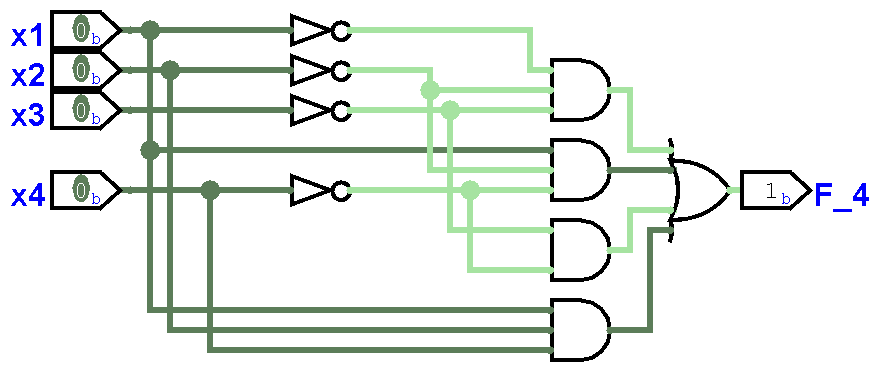
\includegraphics[width=0.7\textwidth]{pics/4f.png}
	\caption*{Рисунок 4 - Схема $F_4$.}
\end{figure}
\newpage

\noindent\textbf{Задание 2}\\

\newpage
\section*{Вывод}
В результате работы разработаны программы для равномерного и оптимального
кодирования данных. Программы корректно обрабатывают входные данные и формируют
коды в соответствии с заданными алгоритмами. Тестирование подтвердило их
корректность и эффективность.\\

\end{document}